\begin{figure}
  \center
  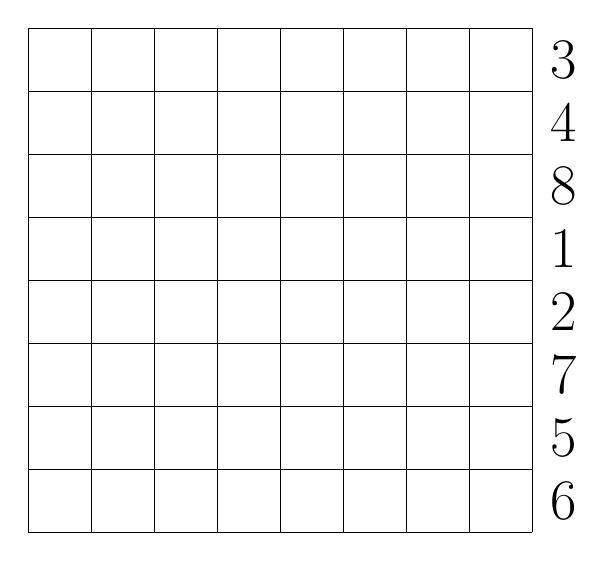
\begin{tikzpicture}[scale = 0.8]
    \foreach \i/\j in {1/3,2/4,3/8,4/1,5/2,6/7,7/5,8/6} {
      \node at (\j - 0.5, 8.5 - \i) {\huge\rook};
      \node at (8.5, 8.5-\i) {\huge\j};
    }
    \draw (0,0) grid (8,8);
  \end{tikzpicture}
  \caption[A permutation corresponding to a rook placement.]{
    An illustration of the rook placement corresponding to the permutation
    $34812756 \in S_8$. A rook is placed in square $(i, \pi(i))$ for each $i$.
  }
  \label{fig:permutationFromRooks}
\end{figure}
